% !TEX program = xelatex
%----------------------- Преамбула -----------------------
\documentclass[ut8x, 14pt, oneside, a4paper]{extarticle}

\usepackage{extsizes} % Для добавления в параметры класса документа 14pt

% Для работы с несколькими языками и шрифтом Times New Roman по-умолчанию
\usepackage[english,russian]{babel}
\usepackage{fontspec}
\setmainfont{Times New Roman}

\usepackage{tocloft}

% ГОСТовские настройки для полей и абзацев
\usepackage[left=30mm,right=10mm,top=20mm,bottom=20mm]{geometry}
\usepackage{misccorr}
\usepackage{indentfirst}
\usepackage{enumitem}
\setlength{\parindent}{1.25cm}
%\setlength{\parskip}{1em} % поменять
%\linespread{1.3}
\renewcommand{\baselinestretch}{1.5}
\setlist{nolistsep} % Отсутствие отступов между элементами \enumerate и \itemize

% Дополнительное окружения для подписей
\usepackage{float}
\usepackage{array}
\newenvironment{signstabular}[1][1]{
	\renewcommand*{\arraystretch}{#1}
	\tabular
}{
	\endtabular
}

\newcommand{\specialcell}[2][c]{%
	\begin{tabular}[#1]{@{}c@{}}#2\end{tabular}}

% Переопределение стандартных \section, \subsection, \subsubsection по ГОСТу;
% Переопределение их отступов до и после для 1.5 интервала во всем документе
\usepackage{titlesec}

\titleformat{\section}[block]
{\bfseries\normalsize}{\thesection}{1em}{}
\titlespacing{\section}{\parindent}{0pt}{1em}

\titleformat{name=\section,numberless}[block]
{\bfseries\normalsize\filcenter}{}{1em}{}
\titlespacing{name=\section,numberless}{0pt}{0pt}{1em}

\titleformat{\subsection}[hang]
{\bfseries\normalsize}{\thesubsection}{1em}{}
\titlespacing\subsection{\parindent}{\parskip}{\parskip}

\titleformat{\subsubsection}[hang]
{\bfseries\normalsize}{\thesubsubsection}{1em}{}
\titlespacing\subsubsection{\parindent}{\parskip}{\parskip}

% Работа с изображениями и таблицами; переопределение названий по ГОСТу
\usepackage{caption}
\captionsetup[figure]{name={Рисунок},labelsep=endash}
%\captionsetup[table]{singlelinecheck=false, labelsep=endash}
\captionsetup[table]{justification=raggedleft, singlelinecheck=false, labelsep=endash}
\captionsetup[tabular]{singlelinecheck=false, labelsep=endash}

\usepackage{graphicx}
\usepackage{diagbox} % Диагональное разделение первой ячейки в таблицах

% Цвета для гиперссылок и листингов
\usepackage{color}

% Гиперссылки \toc с кликабельностью
\usepackage{hyperref}

\hypersetup{
	linktoc=all,
	linkcolor=black,
	colorlinks=true,
}

% Листинги
\setsansfont{Arial}
\setmonofont{Courier New}

\usepackage{color} % Цвета для гиперссылок и листингов
%\definecolor{comment}{rgb}{0,0.5,0}
%\definecolor{plain}{rgb}{0.2,0.2,0.2}
%\definecolor{string}{rgb}{0.91,0.45,0.32}
%\hypersetup{citecolor=blue}
\hypersetup{citecolor=black}

\usepackage{listings}
\usepackage{xcolor}


%\lstdefinelanguage{HTML5}{
	%sensitive=true,
	%keywords={%
		% JavaScript
		%typeof, new, true, false, catch, function, return, null, catch, switch, var, %if, in, while, do, else, case, break,
		% HTML
		%html, title, meta, style, head, body, script, canvas,
		% CSS
		%border:, transform:, -moz-transform:, transition-duration:, %transition-property:,
%		transition-timing-function:
%	},
	% http://texblog.org/tag/otherkeywords/
%	otherkeywords={<, >, \/},
	%ndkeywords={class, export, boolean, throw, implements, import, this},
%	comment=[l]{//},
	% morecomment=[s][keywordstyle]{<}{>},
%	morecomment=[s]{/*}{*/},
%	morecomment=[s]{<!}{>},
%	morestring=[b]',
%	morestring=[b]",
%	alsoletter={-},
%	alsodigit={:}
%}

\lstdefinestyle{customc}{
	breaklines=true,
	frame=single,
	xleftmargin={0.75cm},
	language=C,
	showstringspaces=false,
	basicstyle=\footnotesize\ttfamily,
	keywordstyle=\bfseries\color{green!40!black},
	commentstyle=\itshape\color{purple!40!black},
	identifierstyle=\color{blue},
	stringstyle=\color{orange},
}

\lstset{%
	% Basic design
	backgroundcolor=\color{white},
	basicstyle={\ttfamily},
	frame=single,
	% Line numbers
	xleftmargin={0.75cm},
	numbers=left,
	stepnumber=1,
	firstnumber=1,
	numberfirstline=true,
	% Code design
	identifierstyle=\color{black},
	keywordstyle=\bfseries,
	basicstyle=\footnotesize,
	ndkeywordstyle=\color{black}\bfseries,
	stringstyle=\color{black}\ttfamily,
	commentstyle=\color{black}\ttfamily,
	% Code
	language=C,
	tabsize=2,
	showtabs=false,
	showspaces=false,
	showstringspaces=false,
	extendedchars=true,
	breaklines=true
}


\DeclareCaptionLabelSeparator{line}{\ --\ }
\DeclareCaptionFont{white}{\color{white}}
\DeclareCaptionFormat{listing}{
	\parbox
		{\textwidth}
		{\hspace{15pt}#1#2#3}
}
\captionsetup[lstlisting]{
	format=listing,
	singlelinecheck=false,
	margin=0pt,
	labelsep=line
}

\usepackage{ulem} % Нормальное нижнее подчеркивание
\usepackage{hhline} % Двойная горизонтальная линия в таблицах
\usepackage[figure,table]{totalcount} % Подсчет изображений, таблиц
\usepackage{rotating} % Поворот изображения вместе с названием
\usepackage{lastpage} % Для подсчета числа страниц

\makeatletter
\renewcommand\@biblabel[1]{#1.}
\makeatother

\usepackage{color}
\usepackage{amsmath}
\usepackage{diagbox}
\usepackage{pdfpages}
\usepackage{tabularx}
\usepackage{multirow}
\usepackage{tikz}
\usepackage{pgfplots}
\pgfplotsset{compat=newest}

\begin{document}
	
\includepdf[pages=-]{pdf/title.pdf}
	
	\setcounter{page}{3}
	%\section*{ТЗ}
	%\pagebreak
	
	%\section*{РЕФЕРАТ}
\addcontentsline{toc}{section}{РЕФЕРАТ}

Расчетно-пояснительная записка 37 с., \totalfigures\ рис., \totaltables\ табл., 10 источн., 1 прил.

Ключевые слова: база данных, доступ к данным, система управления базами данных, индекс, таблица, товар, пользователь, приложение, магазин.

Объектом разработки является база данных интернет-магазина электроники.

Область применения -- задача организации работы магазина, осуществляющего розничную торговлю.

Цель работы -- разработать базу данных для организации работы магазина электроники, а также приложение для взаимодействия с ней.

Для достижения поставленной цели требуется решить следующие задачи:

\begin{itemize}[leftmargin=0.7cm + \labelwidth - \labelsep]
	\item[---] формализовать задачу, данные;
	\item[---] проанализировать типы СУБД;
	\item[---] провести обзор существующих аналогов;
	\item[---] описать структуру базы данных;
	\item[---] создать базу данных с ролевой моделью;
	\item[---] спроектировать интерфейс для доступа к БД;
	\item[---] разработать приложение для взаимодействия с созданной БД;
	\item[---] исследовать влияние использования индексов на время выполнения запросов к базе данных.
\end{itemize}

В результате выполнения работы была разработана база данных для организации работы магазина электроники, а также приложение для взаимодействия с ней.

По результатам исследования, использование индексов для столбцов, по значениям которых часто осуществляется поиск данных, позволяет снизить время выполнения запросов к базе данных.

\pagebreak

	\normalsize
	%\renewcommand{\contentsname}{\normalsize\bfseries\centering СОДЕРЖАНИЕ}
	\renewcommand{\contentsname}{\hfill\bfseries\normalsize СОДЕРЖАНИЕ\hfill}
	\renewcommand{\cftaftertoctitle}{\hfill}
	
	\small
	\renewcommand{\cftsecdotsep}{\cftdotsep}
	\tableofcontents
	\normalsize
	\pagebreak
	
	\section*{ВВЕДЕНИЕ}
\addcontentsline{toc}{section}{ВВЕДЕНИЕ}

В настоящее время операционная система Linux прочно занимает лидирующее положение в качестве серверной платформы, опережая многие коммерческие разработки. Тем не менее вопросы защиты информационных систем, построенных на базе этой ОС, не перестают быть актуальными. Существует большое количество технических средств, как программных, так и аппаратных, которые позволяют обеспечить безопасность системы. Это средства шифрования данных и сетевого трафика, разграничения прав доступа к информационным ресурсам, защиты электронной почты, веб-серверов, антивирусной защиты.

Один из способов защиты основан на перехвате системных вызовов операционной системы Linux. Этот способ позволяет взять под контроль работу любого приложения и тем самым предотвратить возможные деструктивные действия, которые оно может выполнить. Также перехват системных вызовов может быть использован для обеспечения возможности мониторинга активности в системе.

Данная работа посвящена исследованию способов перехвата системных вызовов с их последующим логированием и представлением собранных данных в графическом виде для наглядного анализа.

\pagebreak
	\section{Аналитический раздел}

\subsection{Постановка задачи}

В соответствии с заданием на курсовой проект необходимо разработать загружаемый модуль ядра, позволяющий перехватить функции в ядре ОС Linux.
Данная задача выполняется для перехвата системных вызовов sys\_clone() и\\ sys\_execve().

Для решения поставленной задачи необходимо:

\begin{itemize}[leftmargin=0.7cm + \labelwidth - \labelsep]
	\item[---] проанализировать существующие методы перехвата функций в ядре;
	\item[---] описать алгоритм перехвата функций;
	\item[---] реализовать загружаемый модуль ядра;
	\item[---] обеспечить логирование информации о системных вызовах;
	\item[---] представить собранные данные в графическом виде.
\end{itemize}

\subsection{Методы трассировки ядра}

Под трассировкой \cite{ftrace} понимается получение информации о том, что происходит внутри работающей системы. Для этого используются специальные программные инструменты, регистрирующие события в системе.

Программы-трассировщики могут одновременно отслеживать события как на уровне отдельных приложений, так и на уровне операционной системы. Полученная в ходе трассировки информация может оказаться полезной для диагностики и решения многих системных проблем.

Трассировку иногда сравнивают с логированием. Сходство между этими двумя процедурами действительно есть, но есть и различия.

Во время трассировки записывается информация о событиях, происходящих на низком уровне. Их количество исчисляется сотнями и даже тысячами. В логи же записывается информация о высокоуровневых событиях, которые случаются гораздо реже: например, вход пользователей в систему, ошибки в работе приложений, транзакции в базах данных и другие.

\subsubsection{Модификация таблицы системных вызовов}

В ОС Linux все обработчики системных вызовов расположены в таблице sys\_call\_table. Подмена значений в этой таблице \cite{ways} приводит к смене поведения всей системы. Таким образом, сохранив исходный обработчик и подставив в таблицу собственный, можно перехватить любой системный вызов.

Преимуществами этого подхода являются:

\begin{itemize}[leftmargin=0.7cm + \labelwidth - \labelsep]
	\item[---] полный контроль над любыми системными вызовами;
	\item[---] минимальные накладные расходы, нужно один раз изменить таблицу;
	\item[---] не требуется каких-либо конфигурационных опций в ядре, а значит, поддерживается широкий спектр систем.
\end{itemize}

Недостатками являются:

\begin{itemize}[leftmargin=0.7cm + \labelwidth - \labelsep]
	\item[---] необходимость поиска таблицы системных вызовов, обхода защиты от модификации таблицы, безопасного выполнения замены;
	\item[---] невозможность замены некоторых обработчиков из-за оптимизаций при обработке системных вызовов;
	\item[---] перехватываются только системные вызовы.
\end{itemize}

\subsubsection{Linux Security API}

Linux Security API \cite{hookftr} -- специальный интерфейс, созданный именно для перехвата функций. В критических местах кода ядра расположены вызовы\newline security-функций, которые в свою очередь вызывают коллбеки, установленные security-модулем. Security-модуль может изучать контекст операции и принимать решение о ее разрешении или запрете.

К недостаткам этого подхода можно отнести:

\begin{itemize}[leftmargin=0.7cm + \labelwidth - \labelsep]
	\item[---] security-модули являются частью ядра и не могут быть загружены динамически;
	\item[---] в системе может быть только один security-модуль.
\end{itemize}

Таким образом, для использования Security API необходимо пересобирать ядро Linux.

\subsubsection{Kprobes}

Kprobes -- это метод динамической трассировки, с помощью которого можно прервать выполнение кода ядра в любом месте, вызвать собственный обработчик и по завершении всех необходимых операций вернуться обратно. Обработчики получают доступ к регистрам и могут их изменять. Таким образом, можно получить как мониторинг, так и возможность влиять на дальнейший ход работы.

В ядре есть 3 вида kprobes:

\begin{itemize}[leftmargin=0.7cm + \labelwidth - \labelsep]
	\item[---] kprobes -- «базовая» проба, которая позволяет прервать любое место ядра;
	\item[---] jprobes -- jump probe, вставляется только в начало функции и дает доступ к ее аргументам для обработчика, а также работает через setjmp/longjmp, то есть более легковесна;
	\item[---] kretprobes — return probe, вставляется перед выходом из функции и дает доступ к ее результату.
\end{itemize}

Преимущества, которые дает использование kprobes для перехвата:

\begin{itemize}[leftmargin=0.7cm + \labelwidth - \labelsep]
	\item[---] хорошо задокументированный интерфейс, работа kprobes по возможности оптимизирована;
	\item[---] kprobes реализуются с помощью точек останова (инструкции int3), что позволяет перехватить любое место в ядре, если оно известно.
\end{itemize}

К недостаткам kprobes относятся:

\begin{itemize}[leftmargin=0.7cm + \labelwidth - \labelsep]
	\item[---] для получения аргументов функции или значений локальных переменных надо знать, в каких регистрах или где в стеке они лежат, и извлекать их оттуда;
	\item[---] накладные расходы на расстановку точек останова;
	\item[---] jprobes объявлены устаревшими и вырезаны из современных ядер;
	\item[---] kretprobes необходимо хранить исходный адрес возврата, в случае переполнения буфера с адресами kretprobes будет пропускать срабатывания;
	\item[---] kprobes основывается на прерываниях, поэтому для синхронизации все обработчики выполняются с отключенным вытеснением, что накладывает ограничения на обработчики -- в них нельзя выделять много памяти, заниматься вводом-выводом, спать в таймерах и семафорах.
\end{itemize}

\subsubsection{Kernel tracepoints}

Kernel tracepoints -- это метод трассировки ядра, работающий через статическое инструментирование кода.

В качестве преимуществ можно выделить:

\begin{itemize}[leftmargin=0.7cm + \labelwidth - \labelsep]
	\item[---] минимальные накладные расходы -- необходимо лишь вызвать функцию трассировки в нужном месте;
	\item[---] возможность перехвата всех функций.
\end{itemize}

К недостаткам данного метода относится:

\begin{itemize}[leftmargin=0.7cm + \labelwidth - \labelsep]
	\item[---] отсутствие хорошо задокументированного API;
	\item[---] не работает в модуле, если включен CONFIG\_MODULE\_SIG.
\end{itemize}

\subsubsection{Фреймворк ftrace}

Ftrace \cite{docftrace} -- это фреймворк для трассировки ядра на уровне функций. Ftrace был разработан Стивеном Ростедтом и добавлен в ядро в 2008 году, начиная с версии 2.6.27. Работает ftrace на базе файловой системы debugfs, которая в большинстве современных дистрибутивов Linux смонтирована по умолчанию.

Реализуется ftrace на основе ключей компилятора -pg и -mfentry, которые вставляют в начало каждой функции вызов специальной трассировочной функции mcount() или \_\_fentry\_\_(). Обычно, в пользовательских программах эта возможность компилятора используется профилировщиками, чтобы отслеживать вызовы всех функций. Ядро же использует эти функции для реализации фреймворка ftrace.

Для популярных архитектур доступна оптимизация -- динамический ftrace. Суть в том, что ядро знает расположение всех вызовов mcount() или \_\_fentry\_\_() и на ранних этапах загрузки заменяет их машинный код на nop -- специальную ничего не делающую инструкцию. При включении трассировки в нужные функции вызовы ftrace добавляются обратно. Таким образом, если ftrace не используется, то его влияние на систему минимально.

В качестве преимуществ можно выделить:

\begin{itemize}[leftmargin=0.7cm + \labelwidth - \labelsep]
	\item[---] перехват любой функции;
	\item[---] наличие подробной документации;
	\item[---] перехват совместим с трассировкой, с ядра можно снимать полезные показатели производительности.
\end{itemize}

В качестве недостатка можно выделить требования к конфигурации ядра. Для успешного выполнения перехвата функций с помощью ftrace ядро должно предоставлять целый ряд возможностей:

\begin{itemize}[leftmargin=0.7cm + \labelwidth - \labelsep]
	\item[---] список символов kallsyms для поиска функций;
	\item[---] фреймворк ftrace в целом для выполнения трассировки;
	\item[---] опции ftrace, критически важные для перехвата.
\end{itemize}

Обычно ядра, используемые популярными дистрибутивами, все эти опции содержат, так как они не влияют на производительность и полезны при отладке.

\subsubsection{Сравнение методов трассировки ядра}

Сравнение рассмотренных методов приведено в таблице \ref{methods}.

\begin{table}[H]
	\caption{Сравнение методов перехвата функций}
	\label{methods}
	\small
	\begin{tabular}{|c|c|c|c|c|c|}
		\hline
		& \specialcell{Linux\\Security API} & \specialcell{Модиф. таблицы\\сиcтемных вызовов} & kprobes & \specialcell{Kernel\\tracepoints} & ftrace\\ \hline
		\specialcell{Наличие\\документ. API} & - & - & + & - & + \\ \hline
		\specialcell{Динамическая\\загрузка} & - & + & + & + & + \\ \hline
		\specialcell{Перехват всех\\функций} & + & - & + & + & + \\ \hline
		\specialcell{Любая конфигурация\\ядра} & - & + & + & - & - \\ \hline
	\end{tabular}
\end{table}

\pagebreak

В ходе анализа методов перехвата функций для решения поставленной задачи был выбран фреймворк ftrace, так как он позволяет перехватить любую функцию, может быть динамически загружен в ядро, а также обладает хорошо задокументированным API.

\subsection{Средства визуализации лог-файлов}

Визуализация количества вызовов конкретных функций позволяет наглядно оценить состояние системы.
В данной работе для этих целей был выбран Loki \cite{docloki} -- набор компонентов, которые предоставляют широкие возможности по обработке и анализу поступающих данных. В отличие от других подобных систем Loki основан на идее индексировать только метаданные логов -- labels, a сами логи сжимать рядом.

Loki-стек состоит из трех компонентов: Promtail, Loki, Grafana. Promtail собирает логи, обрабатывает их и отправляет в Loki для хранения.

Grafana \cite{docgraf} -- это платформа с открытым исходным кодом для визуализации, мониторинга и анализа данных. Grafana запрашивает данные из Loki и показывает их. Инструмент позволяет создавать панели, каждая из которых отображает определенные показатели в течение установленного периода времени.
Искать по логам можно в специальном интерфейсе Grafana -- Explorer, для запросов используется язык LogQL.

\subsection*{Выводы}

В результате сравнительного анализа методов перехвата функций был выбран фреймворк ftrace, так как он полностью отвечает требованиям реализации.
	\section{Конструкторский раздел}

\subsection{Последовательность преобразований}

Последовательность выполняемых действий в ПО в виде IDEF0 представлена на рисунках \ref{idef1} и \ref{idef2}.

\begin{figure}[H]
	\centering{
		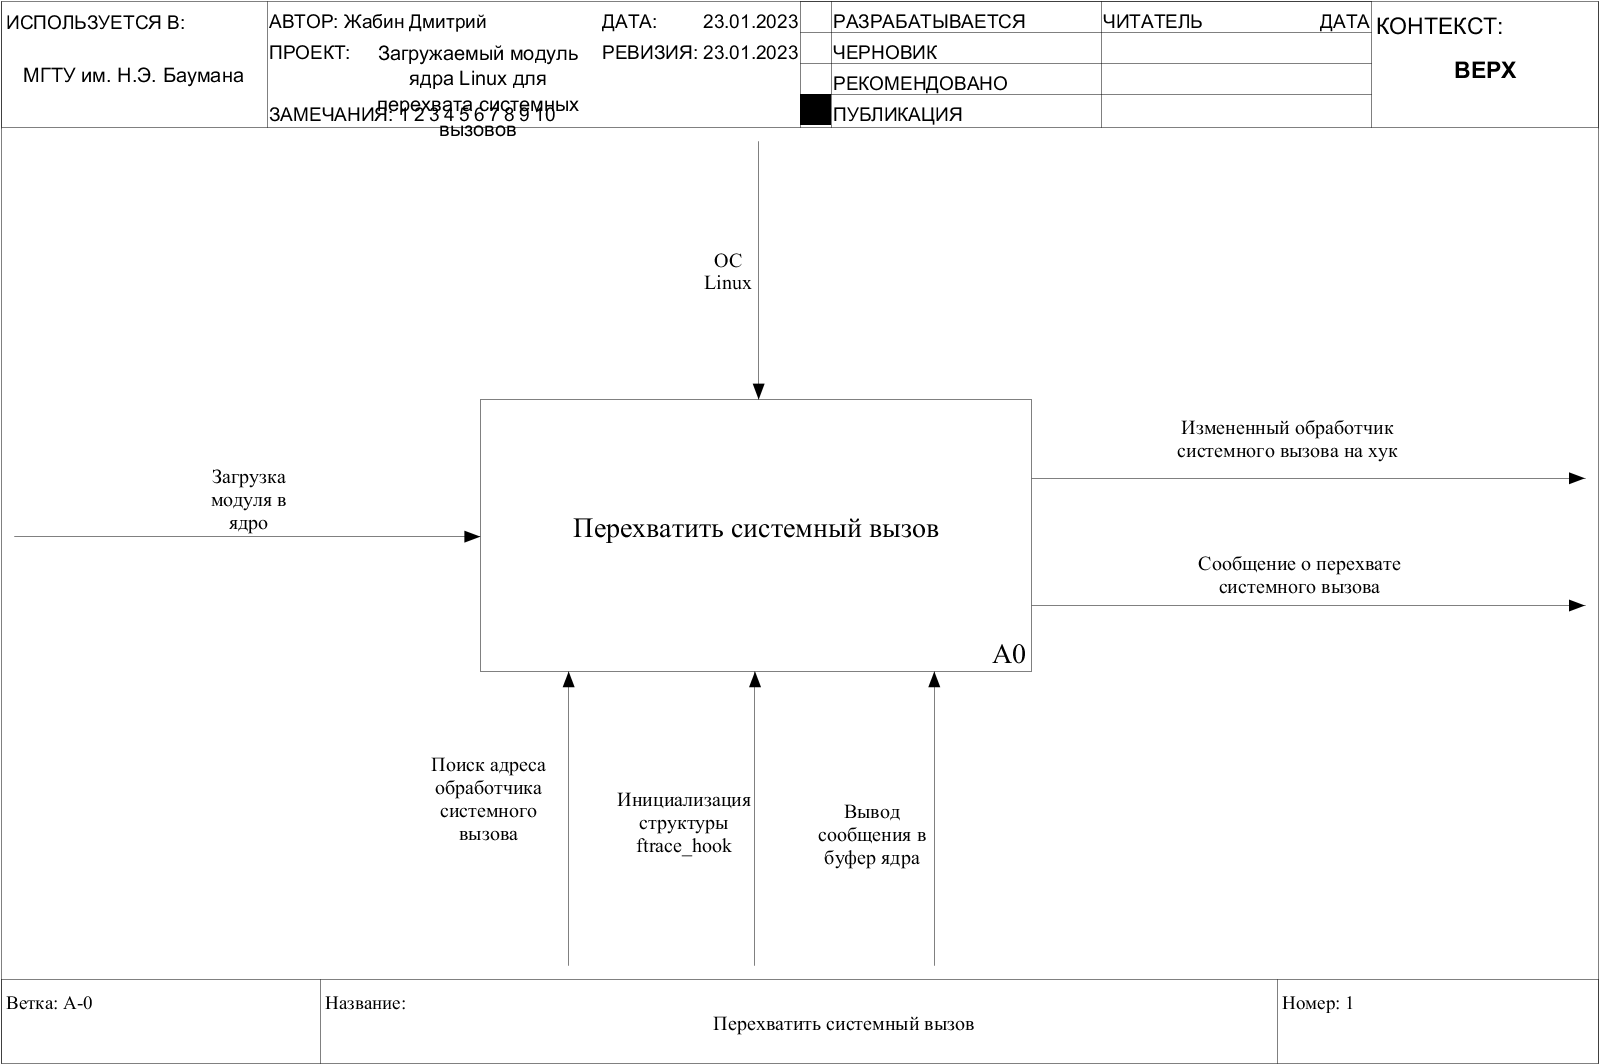
\includegraphics[width=1\textwidth]{img/idef1.png}
		\caption{Последовательность преобразований. Часть 1}
		\label{idef1}}
\end{figure}

\begin{figure}[H]
	\centering{
		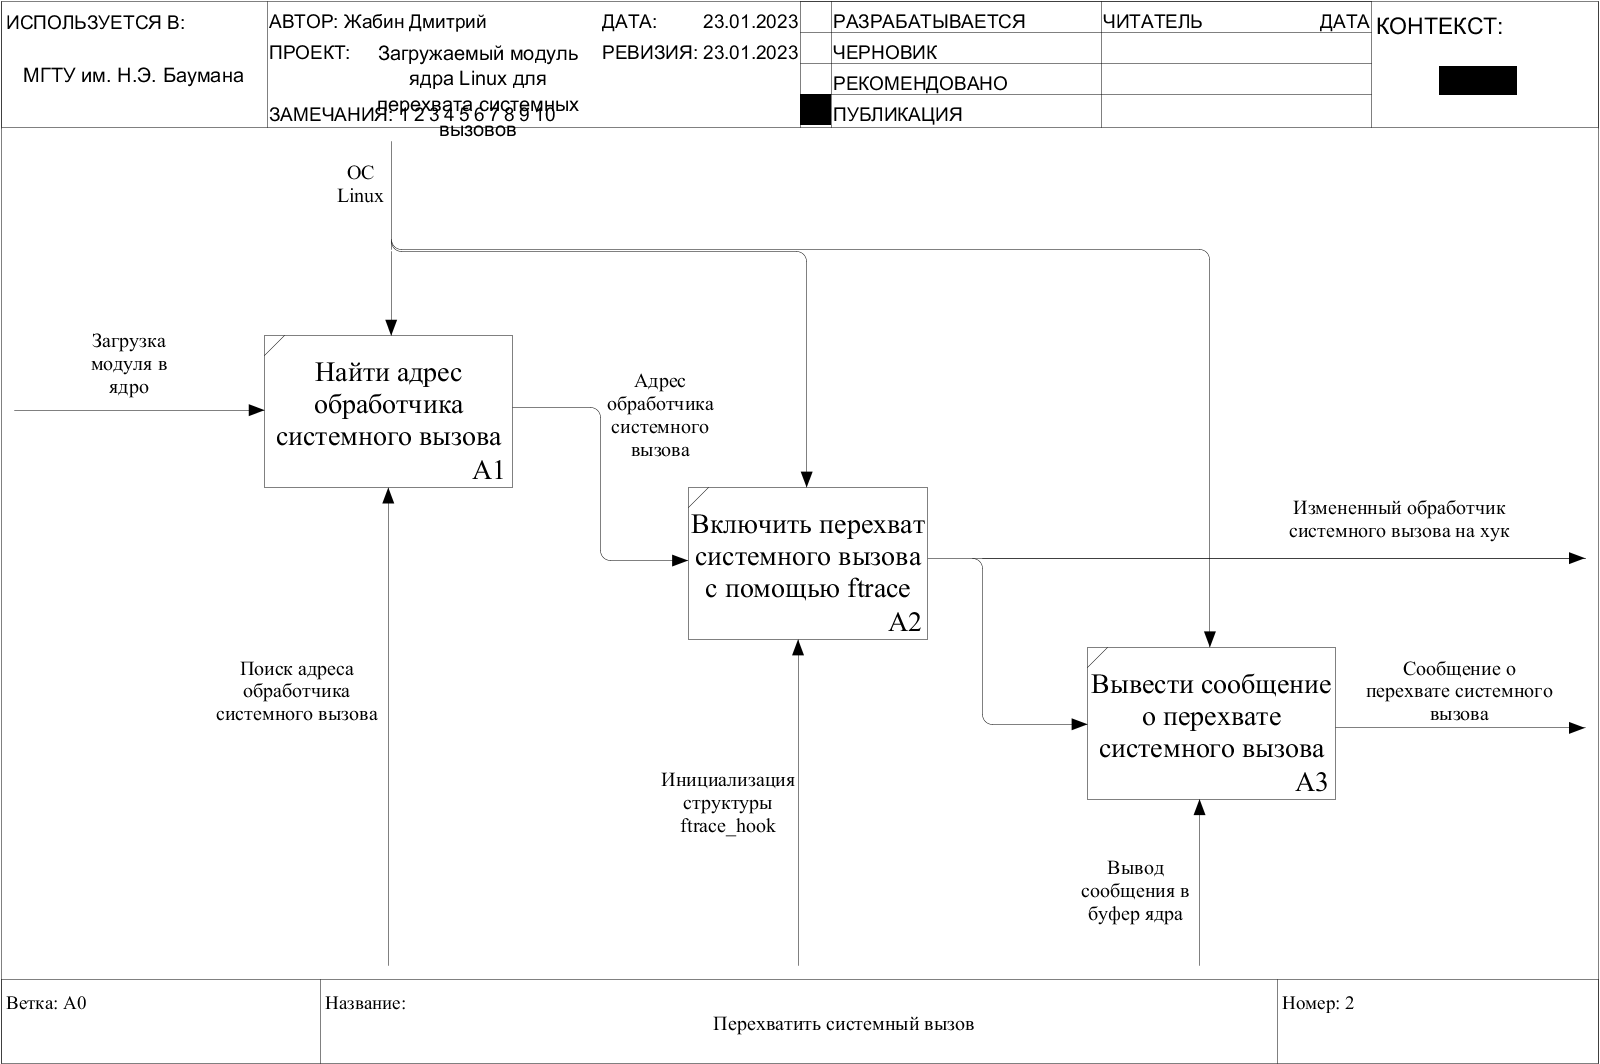
\includegraphics[width=1\textwidth]{img/idef2.png}
		\caption{Последовательность преобразований. Часть 2}
		\label{idef2}}
\end{figure}

\pagebreak

\subsection{Перехват системного вызова}

Схема алгоритма перехвата системного вызова показана на рисунке \ref{hook}.

\begin{figure}[H]
	\centering{
		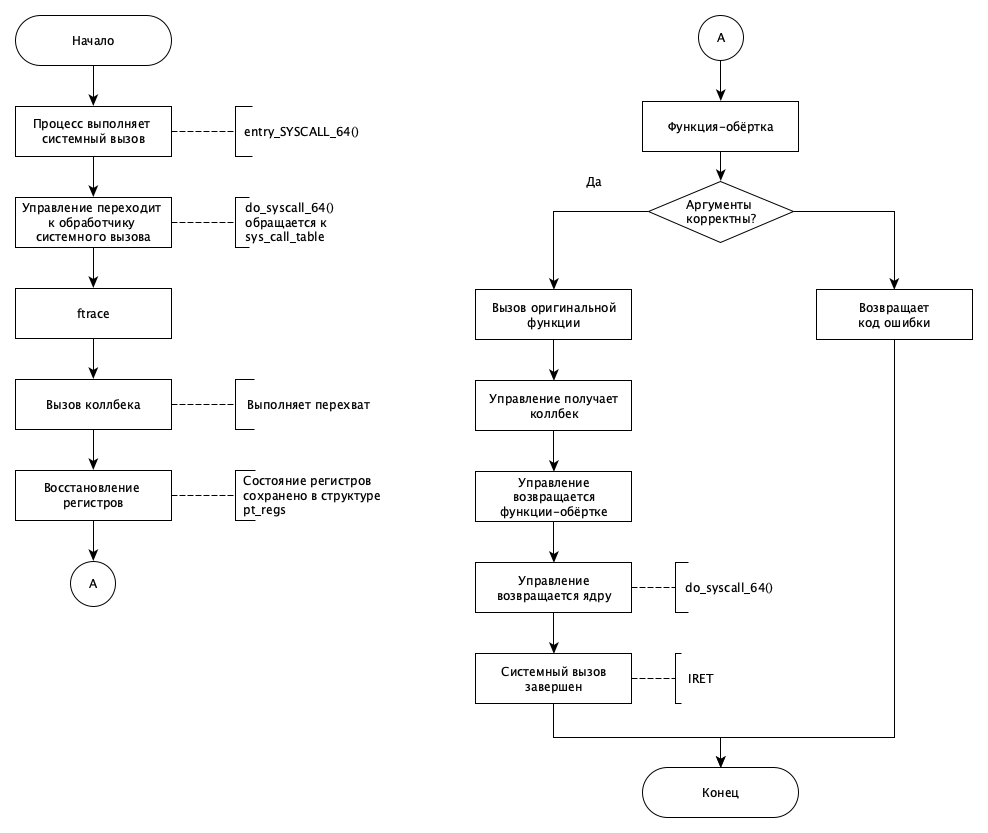
\includegraphics[width=1\textwidth]{img/alg.png}
		\caption{Алгоритм перехвата системного вызова}
		\label{hook}}
\end{figure}

\textbf{Алгоритм перехвата системного вызова}

1. Пользовательский процесс выполняет SYSCALL. С помощью этой инструкции выполняется переход в режим ядра и управление передается низкоуровневому обработчику системных вызовов — entry\_SYSCALL\_64(). Он отвечает за все системные вызовы 64-битных программ на 64-битных ядрах.

2. Управление переходит к конкретному обработчику. Ядро передает управление высокоуровневой функции do\_syscall\_64(). Эта функция в свою очередь обращается к таблице обработчиков системных вызовов sys\_call\_table и вызывает конкретный обработчик по номеру системного вызова -- sys\_execve().

3. Вызывается ftrace. В начале каждой функции ядра находится вызов функции \_\_fentry\_\_(), которая реализуется фреймворком ftrace.

4. Ftrace вызывает разработанный коллбек.

5. Коллбек выполняет перехват.

6. Ftrace восстанавливает регистры. Следуя флагу FTRACE\_SAVE\_REGS, ftrace сохраняет состояние регистров в структуре pt\_regs перед вызовом обработчиков. При завершении обработки ftrace восстанавливает регистры из этой структуры. Коллбек изменяет регистр IP, что в итоге приводит к передаче управления по новому адресу.

7. Управление получает хук. Вместо sys\_execve() управление получает функция hook\_sys\_execve(). При этом остальное состояние процессора и памяти остается без изменений, поэтому хук получает все аргументы обработчика и при завершении вернет управление в функцию do\_syscall\_64().

8. Функция hook\_sys\_execve() вызывает обработчик системного вызова. Она может проанализировать аргументы и контекст системного вызова и запретить или разрешить процессу его выполнение. В случае запрета функция возвращает код ошибки. Иначе же ей следует вызвать обработчик -- sys\_execve() вызывается повторно через указатель orig\_sys\_execve, который был сохранен при настройке перехвата.

9. Управление получает коллбек. Как и при первом вызове sys\_execve(), управление опять проходит через ftrace и передается в коллбек.
 
10. Коллбек ничего не делает, потому что в этот раз функция sys\_execve() вызывается функцией hook\_sys\_execve(), а не ядром из do\_syscall\_64(). Поэтому коллбек не модифицирует регистры и выполнение функции sys\_execve() продолжается как обычно.
 
11. Управление возвращается хуку.

12. Управление возвращается ядру. Функция hook\_sys\_execve() завершается и управление переходит в do\_syscall\_64(), которая считает, что системный вызов был корректно завершен.

13. Управление возвращается в пользовательский процесс. Ядро выполняет инструкцию IRET, системный вызов завершен.

\subsection{Алгоритм включения перехвата}

Ftrace позволяет трассировать функции, но предварительно необходимо найти адрес перехватываемой функции, чтобы вызывать ее.
Также нужно определить коллбек, который ftrace будет вызывать при трассировке функции. В коллбеке нужно заменить значение регистра IP на адрес нового обработчика, таким образом хук перехватит управление.
Для включения перехвата необходимо сначала включить ftrace для перехватываемой функции, а затем разрешить ftrace вызывать коллбек.

Схема алгоритма включения перехвата системного вызова приведена на рисунке \ref{insthook}.

\begin{figure}[H]
	\centering{
		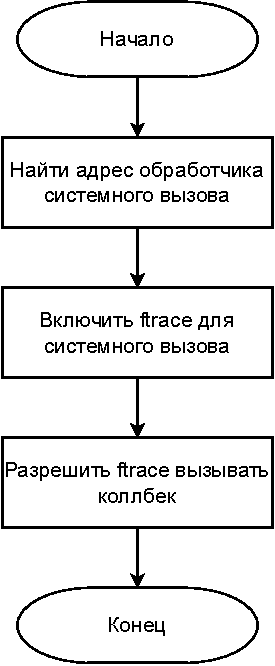
\includegraphics[width=0.3\textwidth]{img/install_hook.pdf}
		\caption{Алгоритм включения перехвата}
		\label{insthook}}
\end{figure}

\subsection{Алгоритм отключения перехвата}

Для отключения перехвата функции необходимо выполнить обратные действия: запретить ftrace вызывать коллбек, а затем отключить ftrace для системного вызова.

Схема алгоритма отключения перехвата системного вызова приведена на рисунке \ref{remhook}.

\begin{figure}[H]
	\centering{
		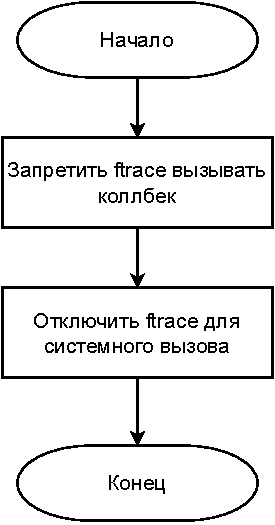
\includegraphics[width=0.3\textwidth]{img/remove_hook.pdf}
		\caption{Алгоритм отключения перехвата}
		\label{remhook}}
\end{figure}

\subsection{Структура ПО}

В состав программного обеспечения входит один загружаемый модуль ядра, который обеспечивает перехват системных вызовов, с последующим сбором информации и ее визуализацией.

\pagebreak

Структура разрабатываемого программного обеспечения представлена на рисунке \ref{structure}.

\begin{figure}[H]
	\centering{
		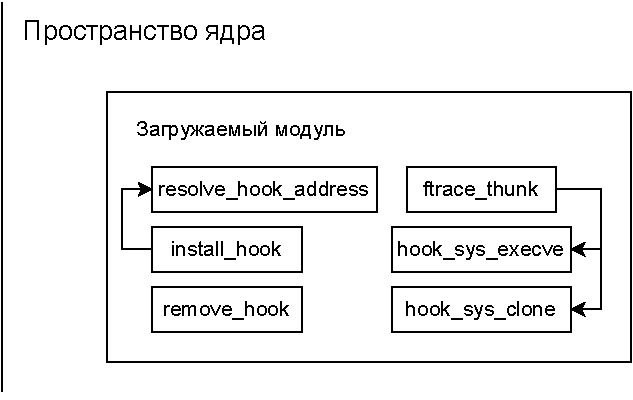
\includegraphics[width=0.7\textwidth]{img/structure.pdf}
		\caption{Структура ПО}
		\label{structure}}
\end{figure}

\subsection{Настройка средств визуализации лог-файлов}

Собранные данные о вызове функций хранятся в лог-файле /var/log/syslog. Для того, чтобы передать их в платформу Grafana для визуализации, необходимо настроить Promtail для считывания данных из лог-файла и их дальнейшей передачи в Loki для хранения.

Фрагмент конфигурационного файла Promtail представлен в листинге \ref{promt}.

\lstinputlisting[
language=C,
firstline=11,
lastline=18,
caption={Конфигурационный файл Promtail},
label={promt},
style=customc
]
{listings/promt.yaml}

\pagebreak

Собранные данные Loki отправляет на порт 3100. Настройка Grafana для прослушивания Loki на этом порту представлена на рисунке \ref{grafset}.

\begin{figure}[H]
	\centering{
		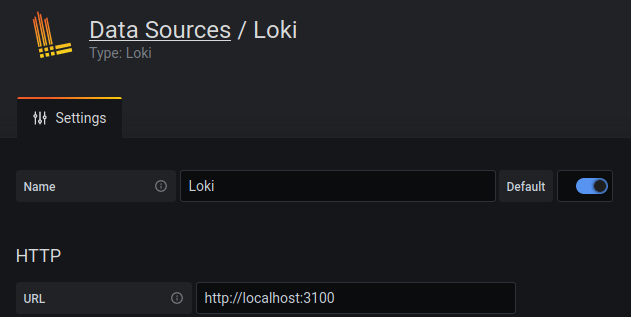
\includegraphics[width=1\textwidth]{img/grafset.png}
		\caption{Настройка Grafana}
		\label{grafset}}
\end{figure}

\pagebreak
	\section{Технологический раздел}

\subsection{Выбор языка и среды программирования}

Исходный код операционной системы Linux написан на языке C, поэтому для реализации загружаемого модуля выбран язык С.

Visual Studio Code~\cite{vscode} предлагает такой инструмент для разработчиков, как IntelliSense.
Это множество функций редактирования кода, таких как, например, code completion, parameter info, quick info, member lists.
Поэтому в качестве среды программирования была выбрана VS Code.


\subsection{Функция включения перехвата}

Для описания перехватываемых функций используется структура struct ftrace\_hook, которая приведена в листинге \ref{struct}.

\lstinputlisting[
language=C,
firstline=21,
lastline=27,
caption={Структура для описания перехватываемой функции},
label={struct},
style=customc
]
{listings/my_hook.c}

Поля приведенной структуры имеют следующее значение: name -- имя перехватываемой функции, function -- адрес хука, вызываемого вместо перехваченной функции, original -- указатель на место, куда будет записан адрес перехватываемой функции, address -- адрес перехватываемой функции.

Для обеспечения перехвата \cite{code} необходимо заполнить только поля name,\newline function, original. Для удобства описания можно использовать макрос, а все перехватываемые функции собрать в массив, что показано в листинге \ref{array}.

\pagebreak

\lstinputlisting[
language=C,
firstline=247,
lastline=256,
caption={Массив перехватываемых функций},
label={array},
style=customc
]
{listings/my_hook.c}

Найти адрес перехватываемой функции можно с использованием krpobes, его получение показано в листинге \ref{addr}.

\lstinputlisting[
language=C,
caption={Получение адреса перехватываемой функции},
label={addr},
style=customc
]
{listings/addr.c}

Для включения перехвата необходимо проинициализировать структуру ftrace\_ops. В ней обязательным полем является лишь func, указывающая на коллбек, но также необходимо установить некоторые важные флаги. Они предписывают ftrace сохранить и восстановить регистры процессора, содержимое которых может измениться в коллбеке.

Функция включения перехвата и коллбек представлены в листингах \ref{install} и \ref{callback} соответственно.

\lstinputlisting[
language=C,
firstline=65,
lastline=93,
caption={Функция включения перехвата},
label={install},
style=customc
]
{listings/my_hook.c}

\lstinputlisting[
language=C,
firstline=55,
lastline=63,
caption={Коллбек, выполняющий перехват},
label={callback},
style=customc
]
{listings/my_hook.c}

Функция отключения перехвата представлена в листинге \ref{remove}.

\lstinputlisting[
language=C,
firstline=95,
lastline=104,
caption={Функция отключения перехвата},
label={remove},
style=customc
]
{listings/my_hook.c}

\subsection{Хуки для перехватываемых функций}

Порядок и типы аргументов и возвращаемого значения хуков должны соответствовать прототипу системного вызова. В хуках происходит вызов обработчика и его логирование.

Реализации хуков для системных вызовов sys\_clone() и sys\_execve() приведены в листингах \ref{clone} и \ref{exec} соответственно.

\lstinputlisting[
language=C,
firstline=155,
lastline=171,
caption={Реализация hook\_sys\_clone()},
label={clone},
style=customc
]
{listings/my_hook.c}

\lstinputlisting[
language=C,
firstline=207,
lastline=222,
caption={Реализация hook\_sys\_execve()},
label={exec},
style=customc
]
{listings/my_hook.c}

\pagebreak

\subsection{Сборка загружаемого модуля ядра}

Функции инициализации и выхода для загружаемого модуля приведены в листинге \ref{lkm}.

\lstinputlisting[
language=C,
firstline=258,
lastline=275,
caption={Функции инициализации и выхода},
label={lkm},
style=customc
]
{listings/my_hook.c}

Сборка загружаемого модуля ядра осуществляется с помощью make-файла, текст которого приведен в листинге \ref{make}.

\lstinputlisting[
language=C,
caption={Make-файл для сборки модуля},
label={make},
style=customc
]
{listings/Makefile}

\pagebreak
	\section{Исследовательский раздел}

\subsection{Примеры работы}

Фрагмент логов, собранных в /var/log/syslog, приведен на рисунке \ref{logs}.

\begin{figure}[H]
	\centering{
		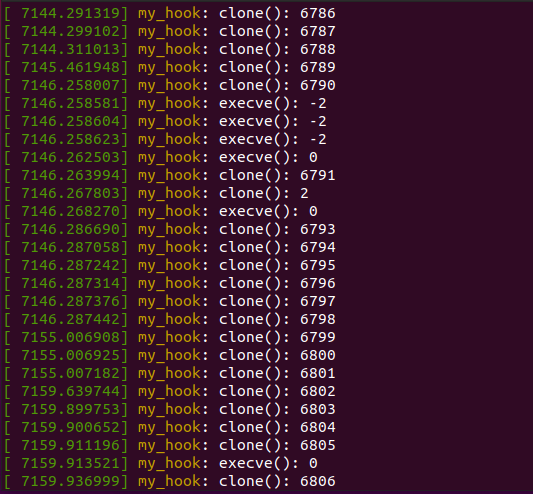
\includegraphics[width=0.8\textwidth]{img/logs.png}
		\caption{Фрагмент /var/log/syslog}
		\label{logs}}
\end{figure}

Результат визуализации собранных данных о системных вызовах с использованием Grafana представлен на рисунках \ref{graf1} и \ref{graf2}.

На первом графике отображены данные за последние 30 минут, сбор метрик проводился каждые 5 минут, а на втором -- за последние 5 минут, сбор метрик проводился каждую минуту. При наведении на график можно увидеть, сколько раз была вызвана каждая функция за последние 10 минут.

\pagebreak

Зеленый график отображает количество вызовов execve(), желтый -- clone().

\begin{figure}[H]
	\centering{
		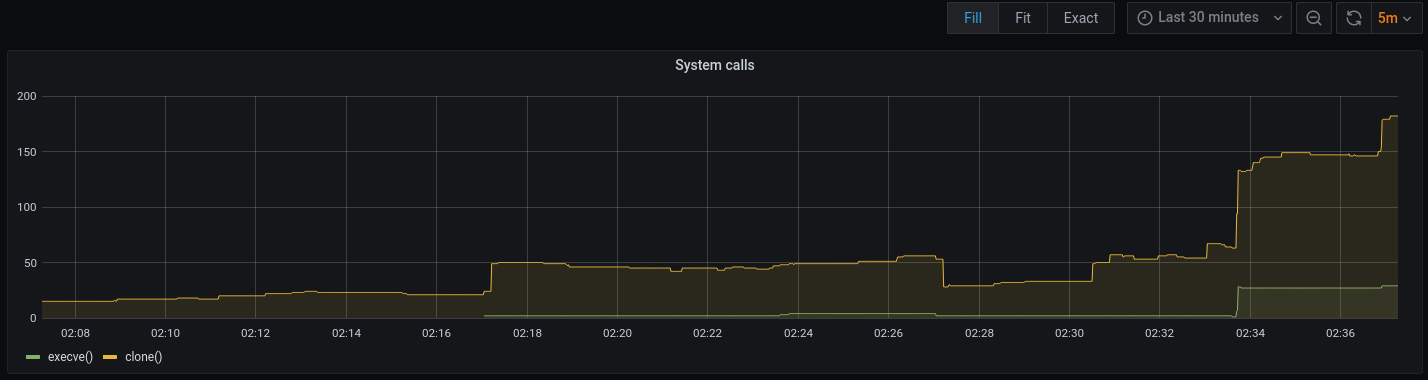
\includegraphics[width=1\textwidth]{img/graf1.png}
		\caption{Вызовы clone() и execve(). Пример 1}
		\label{graf1}}
\end{figure}

\begin{figure}[H]
	\centering{
		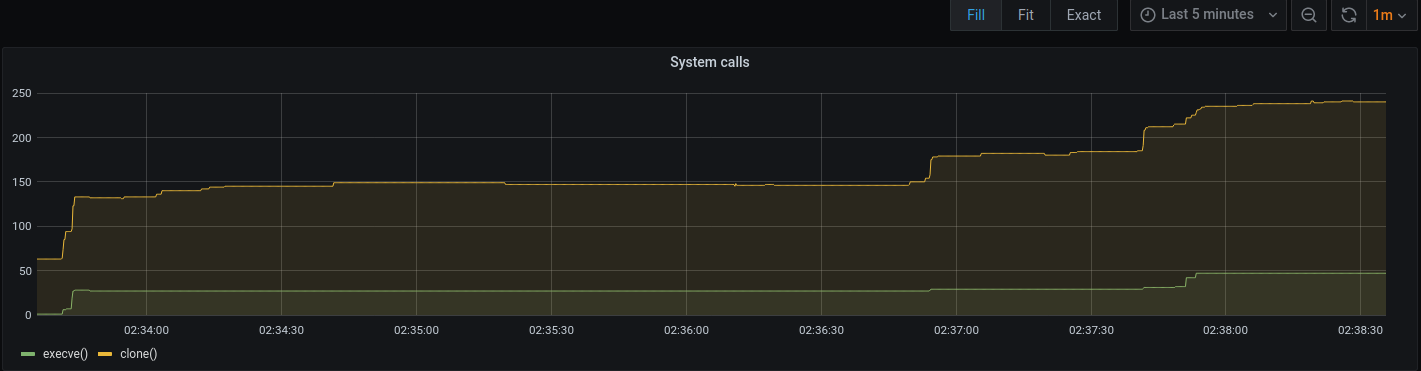
\includegraphics[width=1\textwidth]{img/graf2.png}
		\caption{Вызовы clone() и execve(). Пример 2}
		\label{graf2}}
\end{figure}

\pagebreak
	\section*{ЗАКЛЮЧЕНИЕ}
\addcontentsline{toc}{section}{ЗАКЛЮЧЕНИЕ}

В ходе выполнения курсового проекта разработан загружаемый модуль ядра, позволяющий перехватить системные вызовы sys\_clone() и sys\_execve(). В процессе работы:

\begin{itemize}[leftmargin=0.7cm + \labelwidth - \labelsep]
	\item[---] проанализированы существующие методы перехвата функций ядра;
	\item[---] описан алгоритм перехвата функций;
	\item[---] реализован загружаемый модуль ядра;
	\item[---] обеспечено логирование информации о системных вызовах;
	\item[---] собранные данные представлены в графическом виде.
\end{itemize}

\pagebreak
	\section*{СПИСОК ИСПОЛЬЗОВАННЫХ ИСТОЧНИКОВ}
\addcontentsline{toc}{section}{СПИСОК ИСПОЛЬЗОВАННЫХ ИСТОЧНИКОВ}

\begingroup
\renewcommand{\section}[2]{}
\begin{thebibliography}{}
	
	\bibitem{ftrace}
	Трассировка ядра с ftrace [Электронный ресурс]. -- Режим доступа: https://habr.com/ru/company/selectel/blog/280322/ (дата обращения: 20.11.2022).
	
	\bibitem{ways}
	Linux Rootkits — Multiple ways to hook syscall [Электронный ресурс]. -- Режим доступа: https://foxtrot-sq.medium.com/linux-rootkits-multiple-ways-to-hook-syscall-s-7001cc02a1e6 (дата обращения: 12.12.2022).
	
	\bibitem{hookftr}
	Перехват функций в ядре Linux с помощью ftrace [Электронный ресурс]. -- Режим доступа: https://habr.com/ru/post/413241/ (дата обращения: 20.12.2022).
	
	\bibitem{docftrace}
	Документация ftrace [Электронный ресурс]. -- Режим доступа: https://www.kernel.org/doc/Documentation/trace/ftrace.txt  (дата обращения: 20.12.2022).
	
	\bibitem{cilurik}
	Цилюрик О.И. Модули ядра Linux. Внутренние механизмы ядра [Электронный ресурс]. -- Режим доступа: http://rus-linux.net/MyLDP/BOOKS/Moduli-yadra-Linux/kern-mod-index.html (дата обращения: 15.12.2022).
	
	\bibitem{docloki}
	Документация к Loki [Электронный ресурс]. -- Режим доступа: https://grafana.com/docs/loki/latest/ (дата обращения: 27.12.2022).
	
	\bibitem{docgraf}
	Документация к Grafana [Электронный ресурс]. -- Режим доступа: https://grafana.com/docs/grafana/latest/ (дата обращения: 27.12.2022).
	
	\bibitem{vscode}
	Документация к Visual Studio Code [Электронный ресурс]. -- Режим доступа: https://code.visualstudio.com/docs (дата обращения: 16.12.2022).
	
	\bibitem{code}
	Hooking or Monitoring System calls in linux using ftrace [Электронный ресурс]. -- Режим доступа: https://nixhacker.com/hooking-syscalls-in-linux-using-ftrace/ (дата обращения: 20.12.2022).
	
\end{thebibliography}
\endgroup

\pagebreak
	\section*{ПРИЛОЖЕНИЕ А. Исходный код загружаемого модуля ядра}

\addcontentsline{toc}{section}{ПРИЛОЖЕНИЕ А. Исходный код загружаемого модуля ядра}

\lstinputlisting[
language=C,
firstline=1,
lastline=276,
caption={Исходный код загружаемого модуля ядра},
label={full},
style=customc
]
{listings/fullcode.c}
\end{document}
